\documentclass{article}
\usepackage[dvipdfmx]{graphicx}
\usepackage{here}

\title{README for ssd\_solidangle.cpp}
\author{N. Ozawa}
\date{\today}

\begin{document}

\maketitle

\section{General Idea}
This is a script to 1. Calculate the $\alpha$ detection efficiency of the beam profile monitor and 2. Find the optimum geometry parameters $z_0$ and $x_0$ that maximizes the detection efficiency. Here, "detection efficiency" is defined as the percentage of particles that hit the SSD which are emitted from the surface of the MCP/mesh. In the general literature, "detection efficiency" would be defined as the fraction of $\alpha$ particles that generate a detectable signal at the Si detector out of the number of Fr ions that reached the surface of the MCP/mesh. In our particular case, this efficiency $\varepsilon_{tot}$ could be factorized in the following way:
\begin{eqnarray*}
\varepsilon_{tot} & = & \varepsilon_{mesh} \varepsilon_{decay} \varepsilon_{direction} \varepsilon_{geometry} \varepsilon_{detection}
\end{eqnarray*}
where $\varepsilon_{mesh}$ is the probability that the incoming Fr ion is captured on the mesh surface, $\varepsilon_{decay}$ is the average ratio of Fr ions that decay and emit an $\alpha$ particle, $\varepsilon_{direction} = \frac{1}{2}$ is the ratio of $\alpha$ particles that are emitted in the beamline upstream direction rather than the downstream direction which would be undetectable with the SSD, $\varepsilon_{geometry}$ is the ratio of $\alpha$ particles that enter the SSD holder/box out of the ones that were emitted in the upstream direction, and $\varepsilon_{detection}$ is the ratio of $\alpha$ particles that generate a signal which depends on the detector characteristics. In the script ssd\_solidangle.cpp, only $\varepsilon_{geometry}$ is calculated. This is nearly equivalent to the solid angle $\Omega$ of the hole opened on the lid of the SSD holder/box observed from the center of the MCP. Since the hole is off-axis with respect to the MCP center, it is approximated with $\Omega = 2\pi (1 - \cos{\theta})$, $\cos{\theta} \approx \frac{\sqrt{{z_0}^2+{x_0}^2 }}{\sqrt{\left(\frac{R_{SSD}}{\sqrt{2}}\right)^2 + {z_0}^2 + {x_0}^2}}$. The factor $\sqrt{2}$ for the $R_{SSD}$ is used to approximate the off-axis solid angle with a 45 degree tilt. The meaning of each parameter is to be referenced below. \\

\begin{figure}[H]
  \begin{center}
    \includegraphics[width=8.0cm]{./MCP_caption.png}
    \caption{The planned design for the beam profile monitor.}
    \label{fig:MCP_caption}
  \end{center}
\end{figure}

Figure \ref{fig:MCP_caption} depicts the design of the beam profile monitor. The plate in the center (height $M_H$ and width $M_W$) is the topmost plate holding the MCP. A metal mesh covers this plate which catches the incoming Fr beam. The $\alpha$ particles emitted from the Fr are assumed to emerge from the surface of the plate $\left\{ (x_M,\ y_M,\ z_M)\ |\ x_M = 0,\ -\frac{M_W}{2} \le y_M \le \frac{M_W}{2},\ z_0-\frac{M_H}{2} \le z_M \le z_0+\frac{M_H}{2}\ \right\}$ following the quasi-Gaussian distribution $(X_c, Y_c, \sigma_x, \sigma_y)$ on the MCP coordinates given by the beam simulations. Here, $z_0$ is the distance between the center of the mesh and the lower surface of the lid of the box holding the SSD. The $\alpha$ particle is assumed to be emitted in random directions $\vec{a_M} = (a_x,\ a_y,\ a_z)$, $a_x \ge 0$ from the surface, following a uniform half-sphere direction distribution. \\

The SSD is placed inside the box in the lower right corner in figure \ref{fig:MCP_caption}. A hole of diameter $2R_{{\rm SSD}}$ in the lid of thickness $z_l$ is the entrance for $\alpha$ rays to be detected by the SSD. In the current coordinates, the upper surface of the lid is defined as $\left\{ (x_{lu},\ y_{lu},\ z_{lu})\ |\ z_{lu} = z_l,\ (x_lu - x_0)^2 + y_lu^2 > R_{{\rm SSD}}^2 \right\}$ and the lower surface as $\left\{ (x_{ll},\ y_{ll},\ z_{ll})\ |\ z_{ll} = 0,\ (x_{ll} - x_0)^2 + y_{ll}^2 > R_{{\rm SSD}}^2 \right\}$. Here $x_0$ is the distance between the mesh and the center of the hole in the lid.\\

In this setup, the geometrical parameters $z_0$ and $x_0$ can be adjusted to yield the maximum detection efficiency. In order to analyze this, a method of calculating the detection efficiency is developed in the following way. Note that this method only considers the $\alpha$ particles emitted from the surface of the mesh in the direction of the incoming beam, and enters the SSD box. It does not consider the efficiency of the Fr ions being captured at the mesh, and the detection efficiency of the detector for the $\alpha$ particles that entered the box.\\

For each particle:
\begin{enumerate}
	\item Set point $\vec{P} = (0,\ y_M,\ z_M)$ following a Gaussian random distribution $(X_c,\ Y_c,\ \sigma_X,\ \sigma_Y)$ as $y_M \sim N(X_c,\ \sigma_X)$ and $z_M \sim N(z_0+Y_c,\ \sigma_Y)$, constrained within $-\frac{M_W}{2} \le y_M \le \frac{M_W}{2}$ and $z_0-\frac{M_H}{2} \le z_M \le z_0+\frac{M_H}{2}$ as starting point of the $\alpha$ particle.
	\item Set direction of $\alpha$ particle as $\vec{a_M} = (a_x,\ a_y,\ a_z)$ with $a_x$ as a non-negative random number, and $a_y$ and $a_z$ as random numbers. The random numbers are generated following a normal distribution.
	\item Define $t_u = \frac{z_l - z_M}{a_z}$ so that $\vec{P} + t_u \vec{a_M}$ is on the surface $z = z_l$ i.e. the upper surface of the lid of the SSD box. Similarly, define $t_l = -\frac{z_M}{a_z}$ so that $\vec{P} + t_l \vec{a_M}$ is on the surface $z = 0$ i. e. the lower surface of the lid.
	\item Define $x_{lu} = t_u a_x$, $y_{lu} = y_M + t_u a_y$, $x_{ll} = t_l a_x$, and $y_{ll} = y_M + t_l a_y$. The $\alpha$ particle passes the upper surface of the lid at point $(x_{lu},\ y_{lu},\ z_l)$ and the lower surface of the lid at point $(x_{ll},\ y_{ll},\ 0)$. 
	\item If $(x_{lu} - x_0)^2 + y_{lu}^2 > R_{{\rm SSD}}^2$, the $\alpha$ particle hits the upper lid and does not reach the SSD. Similarly, if $(x_{ll} - x_0)^2 + y_{ll}^2 > R_{{\rm SSD}}^2$, the $\alpha$ particle hits the lid and does not reach the SSD.
\end{enumerate}
Repeat for all the $N_{Fr}$ particles defined and count the number $N_{Detected}$ of them that reached the SSD. The detection efficiency $\varepsilon_i$ for this set $i$ of $N_{Fr}$ particles is defined as $\varepsilon_i = \frac{N_{Detected}}{N_{Fr}}$. This value is expected to be sample-dependent, since the particle positions and directions are randomly selected. In order to obtain a more reliable value, the average of $N_{Average}$ samples is calculated as the final detection efficiency: $\varepsilon = \sum_{i=1}^{N_{Average}} \varepsilon_i$. \\

In the code, the value of $\varepsilon$ is calculated for various combinations of $z_0$ and $x_0$. For the TOF-BPM at CYRIC, $z_0 = 29$ mm and $x_0 = 33$ mm.





\subsection{Generating Random Trajectories}
In the code, random trajectories are defined by giving a random "starting point" 
$$
\vec{P_0} = \left(
\begin{array}{c}
	0 \\
	y_M \\
	z_M
\end{array} \right)
$$
and a random "direction" 
$$
\vec{d} = \left(
\begin{array}{c}
	a_x \\
	a_y \\
	a_z
\end{array} \right)
$$
so that using some parameter $t$, $\vec{P_0} + t\vec{d}$ creates a trajectory of the emitted $\alpha$ particle. Based on the Fr ion simulations, $y_M$ and $z_M$ are assumed to follow a normal distribution. $\vec{d}$ is then given randomly, so that the direction is uniformly distributed on a half-sphere surface in the beamline upstream direction. This could be done by selecting the parameters $a_x$, $a_y$, and $a_z$ randomly, following a normal distribution\cite{Muller1959}. This could be understood in the following way. \\

Suppose $a_x$, $a_y$, and $a_z$ are all generated following a normal distribution
$$
N_k(0,\ R) = \frac{1}{\sqrt{2\pi}R}\exp{\left(-\frac{{a_k}^2}{2R^2}\right)}\, \, \, \, \, (k = x, y, z)
$$
with some positive number $R$. Since all three parameters are individually determined, the set of numbers $(a_x, a_y, a_z)$ are generated following a 3D normal distribution
$$
N_x(0,\ R) N_y(0,\ R) N_z(0,\ R) = \frac{1}{(2\pi)^\frac{3}{2} R^3} \exp{\left(-\frac{{a_x}^2 + {a_y}^2 + {a_z}^2}{2R^2}\right)}.
$$
When we take a sample sphere of ${a_x}^2 + {a_y}^2 + {a_z}^2 = r^2$ where $r$ is some constant, the distribution itself becomes a constant, which corresponds to a uniform distribution over the 3D spherical surface of radius $r$. \\

This is not the case when $\vec{d}$ is generated using uniformly distributed random numbers. Suppose $a_x$,$a_y$, and $a_z$ are generated following a uniform distribution
$$
U_k(0,\ R) = \left\{
\begin{array}{ll}
	\frac{1}{2R} & (-R \le a_k \le R) \\
	0 & ({\rm otherwise})
\end{array} \right. \, \, \, \, \, (k = x, y, z).
$$
Following the same method as above, the set of numbers $(a_x, a_y, a_z)$ follow the distribution
$$
U_x(0,\ R) U_y(0,\ R) U_z(0,\ R) = \left\{
\begin{array}{ll}
	\frac{1}{8R^3} & \left( (-R \le a_x \le R) \cap (-R \le a_y \le R) \cap (-R \le a_z \le R) \right) \\
	0 & ({\rm otherwise})
\end{array} \right. .
$$
This corresponds to a uniform distribution over the volume of a cube, not the surface of a sphere. This is demonstrated using the code random\_tester.cpp producing the follwing scatter plot. When $\vec{d}$ is generated using a uniform distribution, a cube-shaped shadow appears, corresponding to a non-uniformly distributed points on the sphere surface.

\begin{figure}[H]
  \begin{center}
    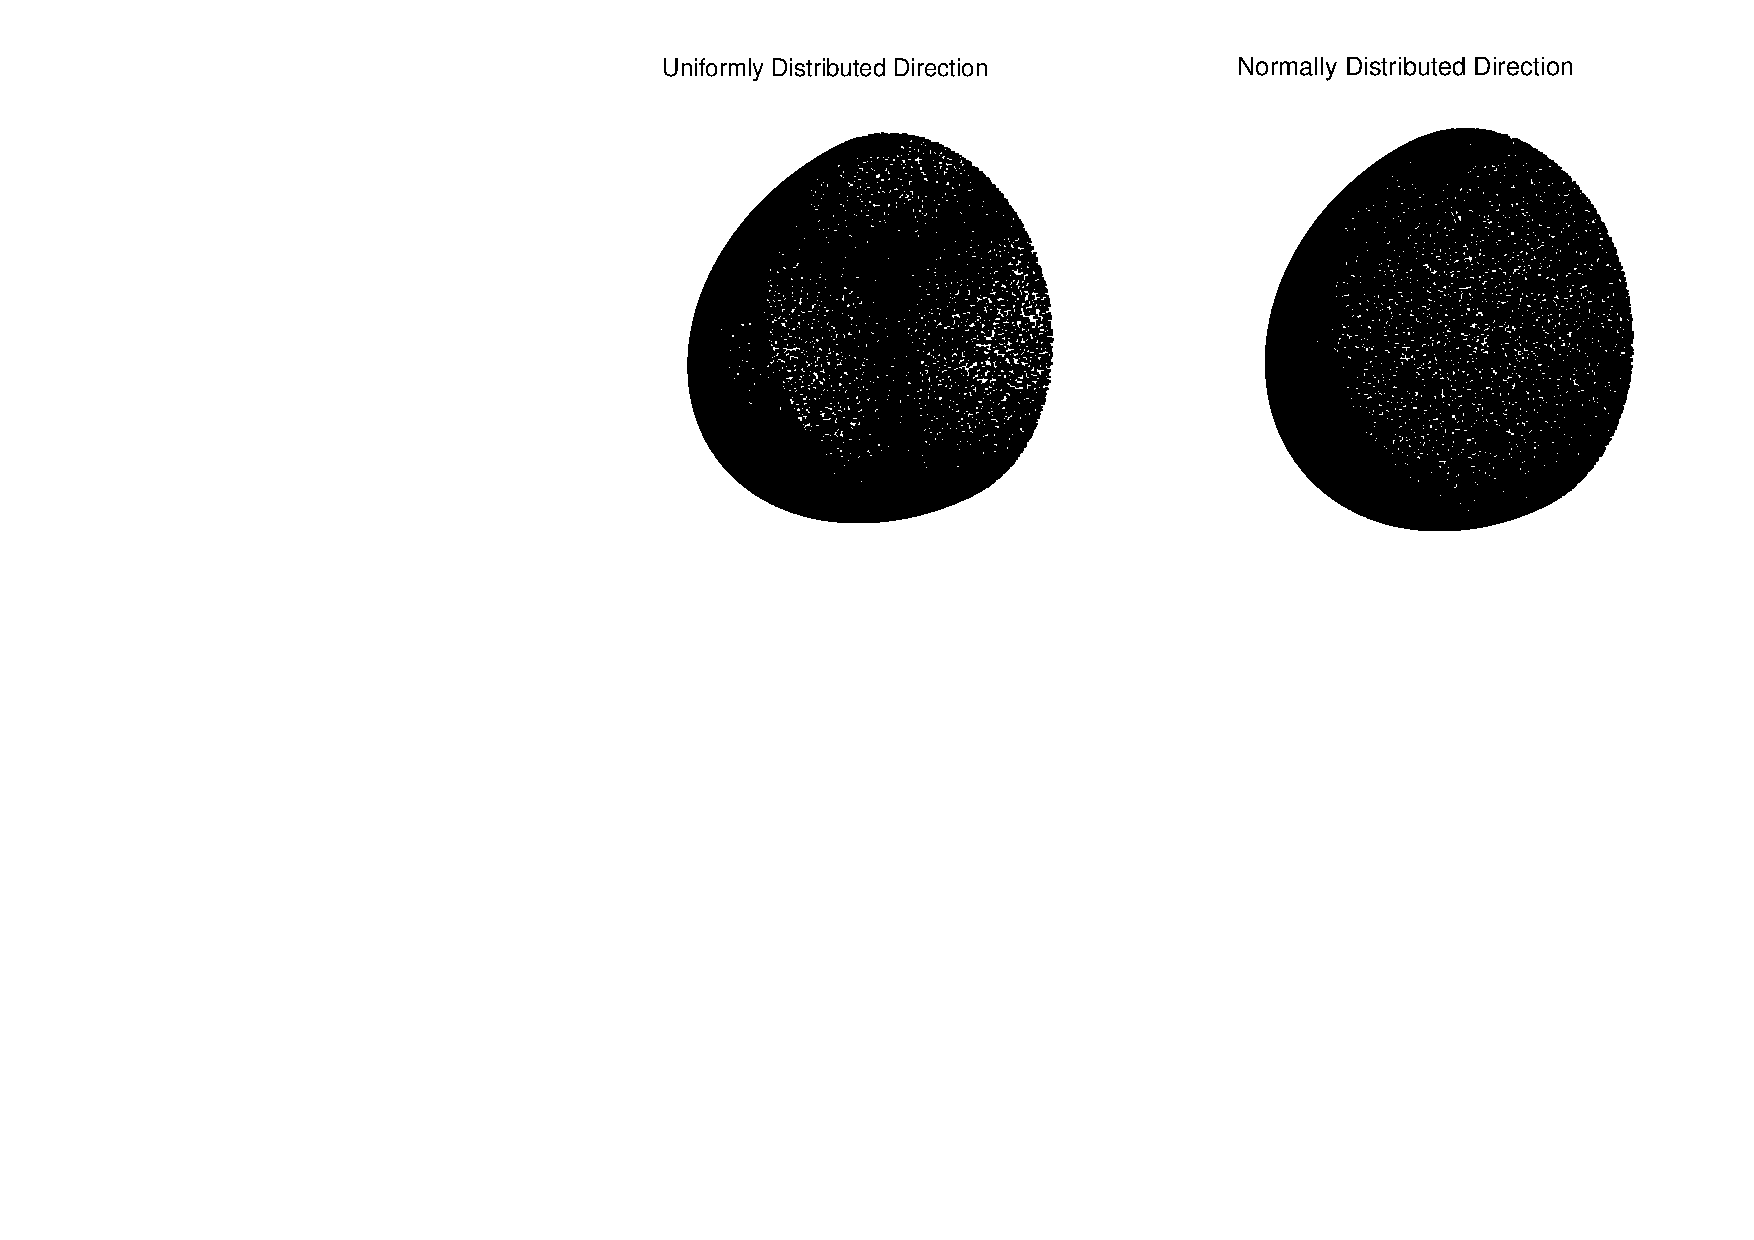
\includegraphics[width=7.0cm,angle=-90]{./random_tester.pdf}
%    \caption{The planned design for the beam profile monitor.}
%    \label{fig:MCP_caption}
  \end{center}
\end{figure}




\subsection{Case with no mesh}
In the case where a mesh is not applied, the Fr ions will be attatched to the surface of the MCP front panel. Since the open-area ratio (OAR) of our MCP is 63\%, approximatly 37\% of the Fr that reached the MCP will be attatched to the surface. This corresponds to the replacement

$$
\varepsilon_{mesh} \rightarrow \varepsilon_{MCP} = 0.37
$$

for the detection efficiency. Furthermore, the calculation method for $\varepsilon_{geometry}$ must be altered so that the $\alpha$ particles originate at the surface of the MCP. As a simple approximation, this could be achieved by just extending the length $X_0$ in the code ssd\_solidangle,cpp. Applying this method, the efficiency of 

$$
\varepsilon_{geometry} = 0.0077
$$

has been obtained.

Therefore, 

$$
\varepsilon_{\alpha} = \varepsilon_{MCP} \varepsilon_{direction} \varepsilon_{geometry} = 0.0014245
$$

is the ratio of the $\alpha$ particles emitted on the MCP-IN surface that reaches the SSD surface.





\section{A much more realistic consideration}

\begin{figure}[H]
  \begin{center}
    \includegraphics[width=7.0cm]{./figures/MCP2_captioned.png}
	  \caption{The geometry of the beam profile monitor around the MCP and SSD. The SSD box contains the SSD with its sensitive side facing upwards, and the ${}^{241}$Am box contains the ${}^{241}$Am $\alpha$ source. Each box has a hole $R_{SSD} = 6.5$ mm and $R_{Am} = 2.5$ mm at the center respectively, so that the $\alpha$ rays can be emitted towards the SSD, and the SSD can catch $\alpha$ rays from the Am source and Fr.}
    \label{fig:MCP2_captioned}
  \end{center}
\end{figure}

As done previously, the center of the MCP-IN surface will be defined as the origin. The $x$ axis is equivalent to the Fr beam upstream direction, i.e. towards the SSD holder, the $z$ axis points towards the ICF152 flange holding the BPM, and the $y$ axis direction is chosen to form a right-handed corrdinate system.

\begin{figure}[H]
  \begin{center}
    \includegraphics[width=7.0cm]{./figures/CoordinateSystem_captioned.png}
	  \caption{The coordinate system defined for this simulation.}
    \label{fig:CoordinateSystem_captioned}
  \end{center}
\end{figure}

Thus, the MCP surface is defined as

$$
MCP_{surface} = \left\{ (x,~y,~z) \right| \left. x = 0,~y^2 + z^2 < R_{MCP}^2 \right\}
$$

where $R_{MCP} = 14~{\rm mm}$ and the SSD sensitive surface is defined as

$$
SSD_{surface} = \left\{ (x,~y,~z) \right| \left. (x - x_0)^2 + y^2 < R_{SSD}^2,~z = -z_0 \right\}.
$$

where $x_0 = 30.8~{\rm mm},~R_{SSD} = 6.5~{\rm mm},~z_0 = 24~{\rm mm}$.



\subsection{$\alpha$ particle emission}

Given the actual geometry of the BPM and the fact that the Fr beam profile can differ greatly from the simulated prediction, a far more general simulation should be done. Practically, $\alpha$ particles could be emitted from five different places:

\subsubsection{Case 1: From the MCP-IN surface}

\begin{figure}[H]
  \begin{center}
    \includegraphics[width=7.0cm]{./figures/EmitCase1.png}
	  \caption{The Fr beam could be stopped at the surface of the MCP (the blue region).}
    \label{fig:EmitCase1}
  \end{center}
\end{figure}

$$
EmitSurface1 = \left\{ (x,~y,~z) \right| \left. x = 0,~y^2+z^2 < R_{MCP}^2 \right\}
$$

\subsubsection{Case 2: From the surface of the MCP lid}

\begin{figure}[H]
  \begin{center}
    \includegraphics[width=7.0cm]{./figures/EmitCase2.png}
	  \caption{The Fr beam could be stopped at the surface of the MCP lid (the blue region).}
    \label{fig:EmitCase2}
  \end{center}
\end{figure}

$$
EmitSurface2 = \left\{ (x,~y,~z) \right| \left. x = T_{lid},~R_{MCP}^2 < y^2+z^2 < R_{MCPlid}^2 \right\}
$$

where $T_{lid} = 3.5$ mm, $R_{MCP} = 14$ mm, $R_{MCPlid} = 25$ mm.



\subsubsection{Case 3: From the surface of the SSD holder}

\begin{figure}[H]
  \begin{center}
    \includegraphics[width=7.0cm]{./figures/EmitCase3.png}
	  \caption{The Fr beam could be stopped at the surface of the SSD holder (the blue region).}
    \label{fig:EmitCase3}
  \end{center}
\end{figure}

\begin{eqnarray*}
	EmitSurface3 & = & \left\{ (x,~y,~z) \right| x = SSDholder_{front},\\
	& & \left( -\frac{W_{SSDholder}}{2} < y < \frac{W_{SSDholder}}{2},~-\frac{H_{SSDholder}}{2} < z < \frac{H_{SSDholder}}{2} \right) \\
	& \cap & \overline{\left( y^2+z^2 < R_{MCP}^2 \right)} \\
	& \cap & \overline{\left( -\frac{W_{SSDboxlid}}{2} < y < \frac{W_{SSDboxlid}}{2}, H_{SSDboxlid} < z < \frac{H_{SSDholder}}{2} \right)} \\
	& \cap & \left. \overline{\left( -\frac{W_{SSDboxlid}}{2} < y < \frac{W_{SSDboxlid}}{2}, -\frac{H_{SSDholder}}{2} < z < -H_{SSDboxlid} \right)} \right\}
\end{eqnarray*}

where $SSDholder_{front} = 16.8$ mm, $W_{SSDholder} = 50$ mm, $H_{SSDholder} = 64$ mm, $W_{SSDboxlid} = 28$ mm, $H_{SSDboxlid} = 23$ mm.



\subsubsection{Case 4: From the surface of the Am box}

\begin{figure}[H]
  \begin{center}
    \includegraphics[width=7.0cm]{./figures/EmitCase4.png}
	  \caption{The Fr beam could be stopped at the surface of the Am box (the blue region).}
    \label{fig:EmitCase4}
  \end{center}
\end{figure}

\begin{eqnarray*}
	EmitSurface4 & = & \left\{ (x,~y,~z) \right| \\
	&  & \left( SSDholder_{front} < x < SSDhole,~-\frac{W_{SSDboxlid}}{2} < y < \frac{W_{SSDboxlid}}{2} \right) \\
	& \cup & \left. \left( (x-x_0)^2+y^2 < R_{SSD}^2 \cap (x-x_0)^2+y^2 > R_{SSD}^2 \right),~z = H_{SSDboxlid} \right\}
\end{eqnarray*}


\subsubsection{Case 5: From the ${}^{241}$Am source itself}

$$
EmitSurface5 = \left\{(x,~y,~,z) \right| \left. (x-x_0)^2 + y^2 < R_{Am}^2, z = z_0 \right\}
$$

where $R_{Am} = 2.5$ mm.



\subsection{$\alpha$ ray hit detection}

The $\alpha$ rays emitted from the five positions listed above could be blocked by the following components before it reaches the SSD sensitive surface. 


\subsubsection{Hit 1: MCP lid side}

\begin{figure}[H]
  \begin{center}
    \includegraphics[width=7.0cm]{./figures/HitCase1.png}
	  \caption{The $\alpha$ particle could be stopped at the side of the MCP hole (the red region).}
    \label{fig:HitCase1}
  \end{center}
\end{figure}

$$
HitSurface1 = \left\{(x,~y,~z) \right| \left. 0 < x < T_{lid},~ y^2+z^2 = R_{MCP}^2 \right\}
$$

\subsubsection{Hit 2: SSD holder back + inner side}

\begin{figure}[H]
  \begin{center}
    \includegraphics[width=7.0cm]{./figures/HitCase2.png}
	  \caption{The $\alpha$ particle could be stopped at the back of the SSD holder and the side of the hole on it (the red region).}
    \label{fig:HitCase2}
  \end{center}
\end{figure}

\begin{eqnarray*}
	HitSurface2 & = & \left\{(x,~y,~z) \right| \\
	& & \left( x=SSDholder_{back}, -\frac{W_{SSDholder}}{2}  < y < \frac{W_{SSDholder}}{2},\right. \\
	& & \left. -\frac{H_{SSDholder}}{2} < z < \frac{H_{SSDholder}}{2}, y^2+z^2 > R_{MCP}^2 \right) \\
	& \cup & \left. \left( y^2+z^2 = R_{MCP}^2, SSDholder_{back} < x < SSDholder_{front} \right) \right\}
\end{eqnarray*}

where $SSDholder_{back} = 13.8$ mm.

\subsubsection{Hit 3: SSD box lid + side}

\begin{figure}[H]
  \begin{center}
    \includegraphics[width=7.0cm]{./figures/HitCase3.png}
	  \caption{The $\alpha$ particle could be stopped at the upper surface of the SSD box and side of its hole (the red region).}
    \label{fig:HitCase3}
  \end{center}
\end{figure}

\begin{eqnarray*}
	HitSurface3 & = & \left\{(x,~y,~z) \right| \\
	& & \left( \left( SSDholder_{front} < x < x_0, -\frac{W_{SSDboxlid}}{2} < y < \frac{W_{SSDboxlid}}{2} \right) \right. \\
	& \cup & \left. \left( (x-x_0)^2+y^2<\left(\frac{W_{SSDboxlid}}{2}\right)^2 \right), (x-x_0)^2+y^2 > R_{SSD}^2, z = H_{SSDboxlid} \right) \\
	& \cup & \left. \left( (x-x_0)^2+y^2 = R_{SSD}^2, -z_0 < z < H_{SSDboxlid} \right) \right\}
\end{eqnarray*}


\begin{thebibliography}{9}
	\bibitem{Muller1959} M. E. Muller, {\it Comm. Assoc. Comp. Mach.} {\bf 2}, 19, (1959).
\end{thebibliography}



\end{document}
